\begin{infocard}{Gráfica de una variación lineal}
    \begin{minipage}[t]{0.8\textwidth}
        Una compañía de pizzas vende la pizza pequeña en \$30 pesos. Cada ingrediente cuesta \$8 pesos.
        Sabemos que el costo de una pizza con 0 ingredientes es de \$30 pesos; una pizza con 1 ingrediente cuesta \$8 pesos más,
        es decir, \$38 pesos, y así sucesivamente. A continuación mostramos una tabla que exhibe este hecho:

        \begin{table}[H]
            \rowcolors{2}{colorrds!10}{lightgray!10}
            \centering
            \caption{Costo de una pizza pequeña según la cantidad de ingredientes}
            \label{tab:pizza_ingredientes}
            \begin{tabular}{|c|c|c|}
                \toprule
                \rowcolor{colorrds!80}
                \textbf{\color{white}Ingredientes} & \textbf{\color{white}Costo} & \textbf{\color{white}Coordenada} \\\midrule
                0                                  & \$30                        & $(0,30)$                         \\\hline
                1                                  & \$38                        & $(1,38)$                         \\\hline
                2                                  & \$46                        & $(2,46)$                         \\\hline
                3                                  & \$54                        & $(3,54)$                         \\\hline
                4                                  & \$62                        & $(4,62)$                         \\\hline
                \bottomrule
            \end{tabular}
        \end{table}
        Podemos utilizar estos pares ordenados para crear la gráfica de la Figura \ref{fig:20230320232504}.
    \end{minipage}\hfill
    \begin{minipage}[t]{0.2\textwidth}
        \begin{figure}[H]
            \centering
            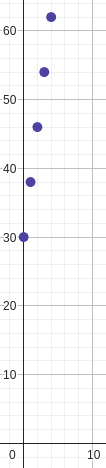
\includegraphics[width=0.5\linewidth]{../images/20230320232504}
            \caption{}%Gráfica de la relación entre la cantidad de ingredientes y el costo en una pizza pequeña.}
            \label{fig:20230320232504}
        \end{figure}
    \end{minipage}

\end{infocard}



